%%%%%%%%%%%%%%%%%%%%%%%%%
% Imports and Setup     %
%%%%%%%%%%%%%%%%%%%%%%%%%

\input{../lib/hw-setup/tex/HWSetup}
\input{../lib/hw-setup/tex/EngBindings}

\fancyhead[C]{}
\fancyhead[R]{\hyperlink{tableofcontents}{\hmwkClass\ (\hmwkClassInstructor,\ \hmwkClassTime): \hmwkTitle}}
\fancyheadwidth[L]{0.5\headwidth}
\fancyheadwidth[C]{0.0\headwidth}
\fancyheadwidth[R]{0.5\headwidth}

%%%%%%%%%%%%%%%%%%%%%%%%%
% Homework Details      %
% - Title               %
% - Subtitle            %
% - Due Date            %
% - Due Time            %
% - Course              %
% - Section Time        %
% - Instructor          %
% - Author              %
% - Submission Time     %
%%%%%%%%%%%%%%%%%%%%%%%%%

\hwkTitle{Lab04}
\hwkSubTitle{Particle Imaging Velocimetry}
\hwkDueDate{2026-04-03}
\hwkDueTime{23:59:00}
\hwkClass{ENAE464 - 0202}
\hwkClassTime{14:00:00}
\hwkInstructor{Dr. Silbaugh}
\hwkAuthor{Mikołaj Kostrzewa \& Vai Srivastava}
\hwkCompletionDate{
        Experiment Performed: \DTMdate{2026-03-27}\\
        Report Submitted: \DTMtoday
}

\addbibresource{./references.bib}

\begin{document}

\hypertarget{titlepage}{\maketitle}
\thispagestyle{empty}

\pagebreak

%%%%%%%%%%%%%%%%%%%%%%%%%
% Letter of Transmittal %
%%%%%%%%%%%%%%%%%%%%%%%%%

\thispagestyle{empty}

\DTMtoday

\vspace{5.0ex}

Enclosed is the technical report for the \textit{Particle Imaging Velocimetry} laboratory experiment. This report presents the experimental methodology, results, and analysis of flow characteristics and imaging effects for a P.I.V. technique on the wake downstream of a circular cylinder.

Please feel free to contact us with any questions regarding the contents of this report.

\vspace{5.0ex}

Respectfully,

Mikołaj Kostrzewa \& Vai Srivastava

%%%%%%%%%%%%%%%%%%%%%%%%%
% Table of Contents     %
%%%%%%%%%%%%%%%%%%%%%%%%%

\pagebreak

\thispagestyle{empty}
\hypertarget{tableofcontents}{\tableofcontents}

\renewcommand{\listfigurename}{Figures}
\listoffigures

\renewcommand{\listtablename}{Tables}
\listoftables

\renewcommand{\listlistingname}{Listings}
\listoflistings

\newpage
\pagenumbering{arabic}

%%%%%%%%%%%%%%%%%%%%%%%%%
% Report                %
%%%%%%%%%%%%%%%%%%%%%%%%%

\section{Abstract} \label{sec:abstract}

% TODO:

\section{Introduction} \label{sec:introduction}

% TODO:

\subsection{Theoretical Background} \label{sec:introduction/theory}

% TODO:

\subsection{Objectives} \label{sec:introduction/objectives}

% TODO:
The specific objectives of this experiment are:
\begin{enumerate}
    \item foo
\end{enumerate}

\section{Methodology} \label{sec:methodology}

\subsection{Experimental Apparatus} \label{sec:methodology/apparatus}

% TODO:

\begin{figure}[H]
    \centering
    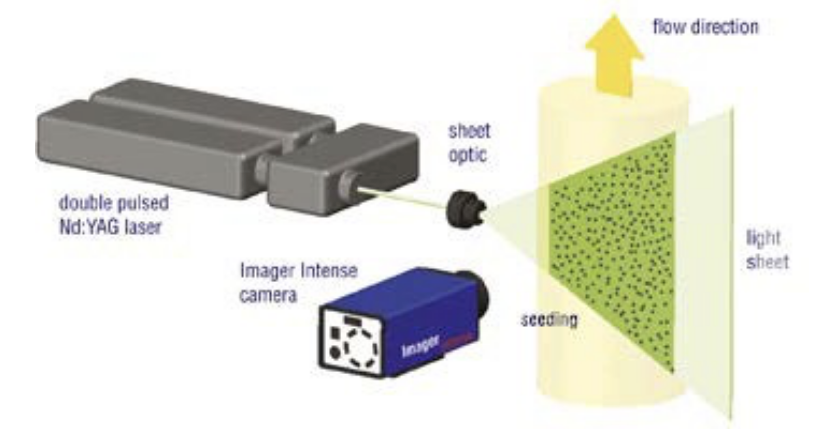
\includegraphics[width=0.65\linewidth]{../assets/PIV-diagram.png}
    \caption{foo}
    \label{fig:procedures/apparatus/piv-diagram}
\end{figure}

\subsection{Operating Procedure} \label{sec:methodology/procedure}

% TODO:

\section{Results} \label{sec:results}

\subsection{Flow Velocity} \label{sec:results/flow-velocity}

% TODO:
% measured flow velocity
% calculations of the incoming water flow speed \(\bar{U}_{\infty}\)

\subsection{Reynolds Number} \label{sec:results/reynolds-number}

% TODO:
% reynolds number
% calculations of the appropriate reynolds number for the water flow over the cylinder

\subsection{Velocity Fluctuation} \label{sec:results/velocity-fluctuation}

% TODO:
% plot \(y\)-velocity fluctuation in the vicinity of \((x, y)=(0,0)\) as a function of time

\subsection{Expected Shedding Frequency} \label{sec:results/expected-shedding-frequency}

% TODO:
% expected shedding frequency and strouhal number
% look up the preffered strouhal number for your case and, from this, estimate the shedding frequency in Hz

\subsection{Stokes Number} \label{sec:results/stokes-number}

% TODO:
% stokes number for visualization
% using the expected shedding frequency as the inverse of the characteristic flow time scale (i.e., \(f_{\text{shedding}}=U/L\) ), calculate the stokes number for the particle seeding

\section{Analysis and Discussion} \label{sec:analysis}

\subsection{Measured Shedding Frequency} \label{sec:analysis/measured-shedding-frequency}

% TODO:
% measured shedding frequency
% from the velocity fluctuation chart, fit a sinusoid to estimate the measured vortex shedding frequency

\subsection{Comparison to Theory} \label{sec:analysis/theory-comparison}

% TODO:
% compare the measured vortex shedding frequency with the expected value
% (these should be close, i.e. not \(\sim\) order of magnitude different)

\section{Summary and Conclusions} \label{sec:summary}

% TODO:

\section{References} \label{sec:references}

\printbibliography[heading=none]

\section{Appendices} \label{sec:appendices}

\subsection{Data} \label{sec:appendices/data}

For the sake of brevity, the raw measurement data will not be displayed in this report. However, in the spirit of completeness, the repository containing the complete data, source code, and notes for this report can be found at \href{https://www.github.com/vaisriv/enae464-lab04}{github:vaisriv/enae464-lab04}.

\subsection{Code} \label{sec:appendices/code}

Similarly, only the code files that are key to the analysis are included below, and can be accessed in full in the aforementioned \href{https://www.github.com/vaisriv/enae464-lab04}{GitHub repository}.

\begin{codeblock}
    \centering
    \caption{Index File}
    \mintinline{bash}{./src/index.py}
    \inputminted{python}{../src/index.py}
    \label{lst:code/index}
\end{codeblock}

% render all references
\nocite{*}

\end{document}
